\documentclass[12pt,center]{beamer}

%%%%%%%%%%% Lo que viene  a continuacion es el tipo de presentacion que quieres, 
% las presentaciones se llaman con nombres de ciudades puedes cambiarlas y tomar
%%%%%%%%la que mas te guste.
\mode<presentation> {
  %\usetheme{Frankfurt}
  %\usetheme{Warsaw}
  %\usetheme{Darmstadt}
  \usetheme{Dresden}
  %\usetheme{Singapore}
  %\usetheme{Bergen}
  %\usetheme{Boadilla}
  %\usetheme{BerKeley}
  \setbeamercovered{transparent}
  %\setbeamertemplate{background canvas}[vertical shading][bottom=red!20,top=yellow!30]
%   \setbeamertemplate{headline}{}
%%%%%%%%%%%%%%%%%%%%%%%%%%%%%%%%%%
%%%%%%% aqui vienen los colores

  %\usecolortheme{crane}
  %\usecolortheme{seahorse}
  \usecolortheme{whale}
  %\usecolortheme{rose}
  %\usecolortheme{orchid}
} \usepackage{alltt}



%%%%%%%los paquetes. 
\usepackage{amssymb,amsmath,latexsym}
%\usepackage[mathcal]{euscript}
%\usepackage[polish]{babel}
%\usepackage{dsfont}
%\usepackage[normalem]{ulem}
\usepackage{enumerate}
%\usepackage[all,2cell,dvips]{xy} \UseAllTwocells \SilentMatrices

\usepackage{verbatim}
\usepackage{float}

\usepackage[utf8]{inputenc}
\usepackage{url}
\usepackage{makeidx}
\usepackage[procnames]{listings}
\usepackage{color}
\usepackage{graphicx} % graficos
\usepackage{subfig}
\usepackage{tabularx}
%\usepackage{subcaption}
\captionsetup{compatibility=false}
\usepackage[export]{adjustbox}
\usepackage[spanish]{babel}
\usepackage{mathtools}
\usepackage{svg}

\newcommand{\subitem}{\par\qquad}

\title{Transferencia de Estilo en Fotografias mediante Redes Neuronales Convolucionales}
%
%
\author{Ariel Wolfmann}

%
\institute{Facultad de Matemática, Astronomía, Física y Computación\\
	  Universidad Nacional de Córdoba}

\date{28 de Julio, 2017}


\begin{document}
%%%%%%%%%%%%%%%%%%%%%%%%%%%PAGINA DEL TITULO
\begin{frame}
  \titlepage
\end{frame}

%%%%%%%%%%%%%%%%%  tODO LO QUE QUIERAS PONER EN LOS FRAMES.
\begin{frame}
  \frametitle{Agenda}
  \tableofcontents[pausesections]
\end{frame}
  %  \tableofcontents[pausesections]
%   %You might wish to add the option [pausesections]


%%%%%%%%%%%%%%%%%%%%%%%% EFDs & Algebraic Functions %%%%%%%%%%%%%%%%%%%%%%%%%%%%
\section{Introducción}
\begin{frame}
  \frametitle{Contexto}
  Aplicaciones de efectos en fotografias:
    \begin{figure}[H]
      \begin{center}
	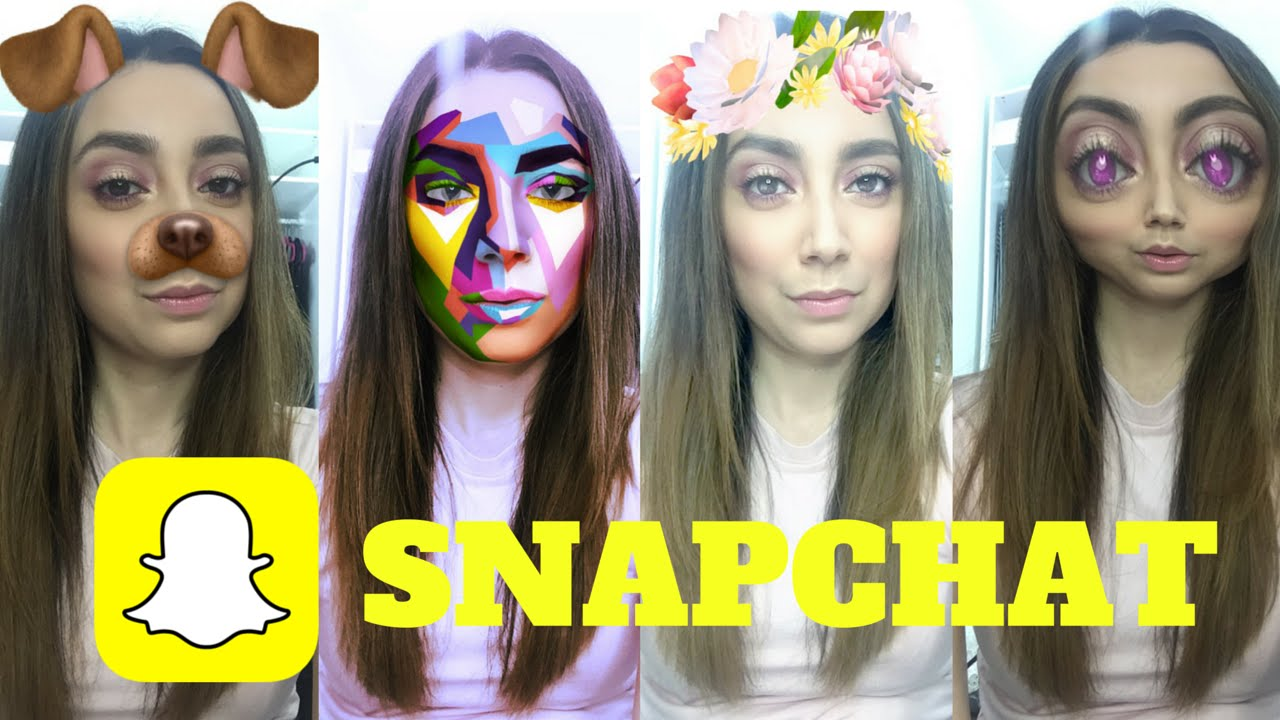
\includegraphics[width=0.8\linewidth]{./img/filtro_snapchat.jpg}
      \end{center}
    \end{figure}
\end{frame}	

\begin{frame}
  \frametitle{Como se representa una imágen}
  Arreglo de píxeles ordenados
    \begin{figure}[H]
      \begin{center}
	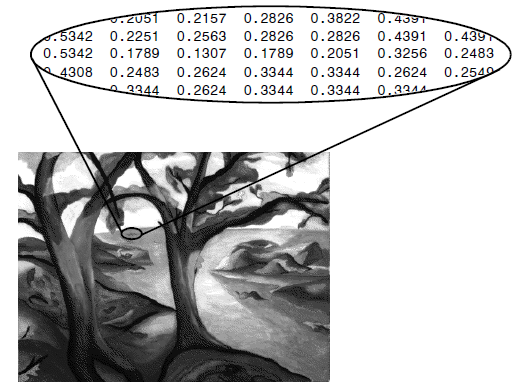
\includegraphics[width=0.8\linewidth]{./img/image_pixel.png}
      \end{center}
    \end{figure}
\end{frame}
  
\begin{frame}
  \frametitle{Aprendizaje automatico en vision por computadoras}
  \begin{itemize}
    \item \textbf{Vision por computadoras} (Computer Vision): Comprensión de alto nivel sobre imágenes digitales, busca automatizar tareas del sistema visual humano.
    \item \textbf{Aprendizaje automático} (Machine Learning): Algortimos que otorgan a las computadoras la habilidad de aprender y hacer predicciones sobre los datos de entrada. 
  \end{itemize}

  
    \begin{figure}[H]
      \begin{center}
	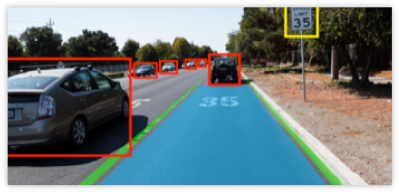
\includegraphics[width=0.8\linewidth]{./img/nvidia_car_detection.png}
      \end{center}
      \caption{Vehiculos autónomos}
    \end{figure}    
\end{frame}
  
\begin{frame}
  \frametitle{Transferencia de estilo}
  A partir de una imagen de contenido y una imagen de estilo se genera una nueva imagen que combina ambos.
  \begin{figure}[h]
    \begin{center}
      \subfloat[Imagen de Estilo]{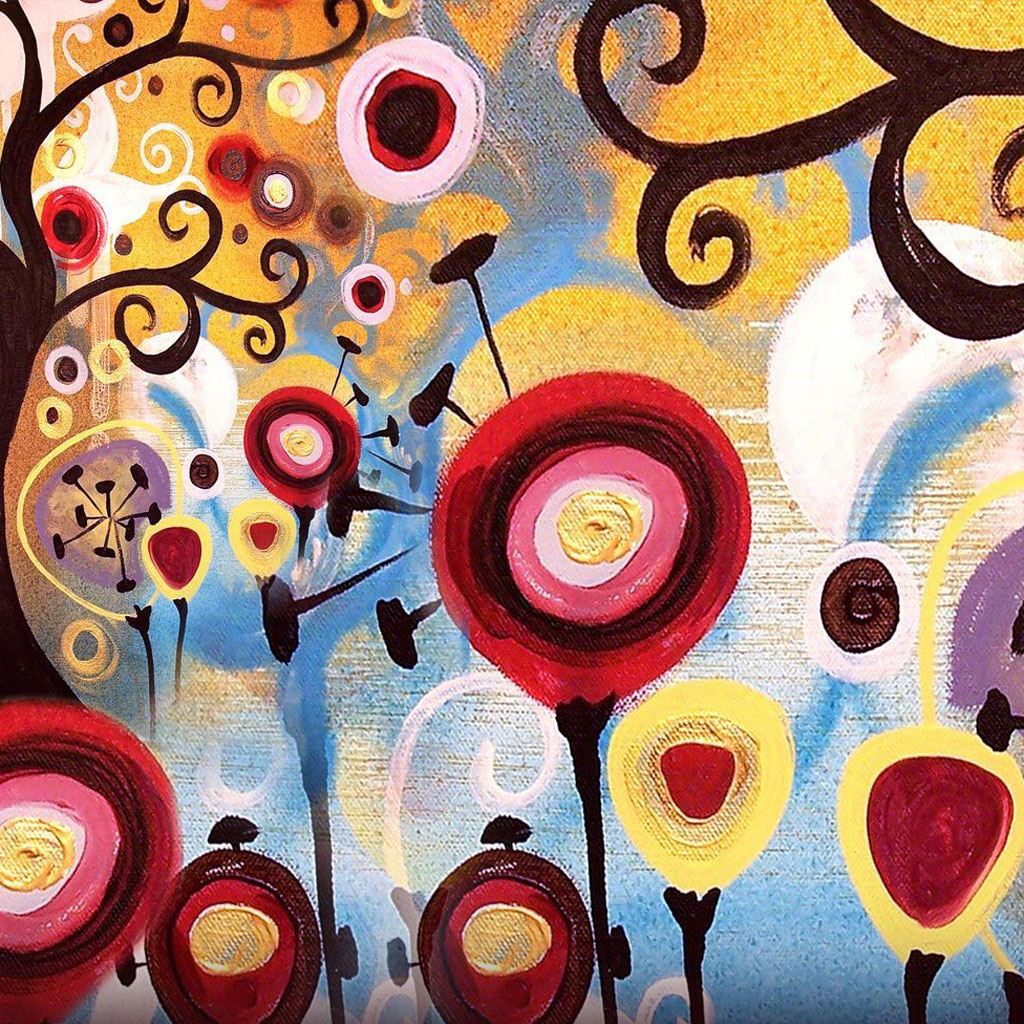
\includegraphics[height=0.20\textheight]{./img/jhonson_style_candy.jpg}}\\
      \subfloat[Imagen de Contenido]{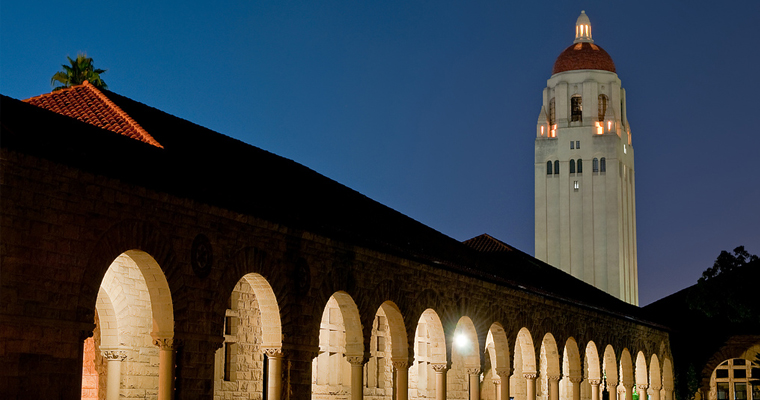
\includegraphics[height=0.20\textheight]{./img/jhonson_content_tower.jpg}}\\ 
      \subfloat[Resultado obtenido transfiriendo el estilo de la obra de arte a la imagen de contenido]
	{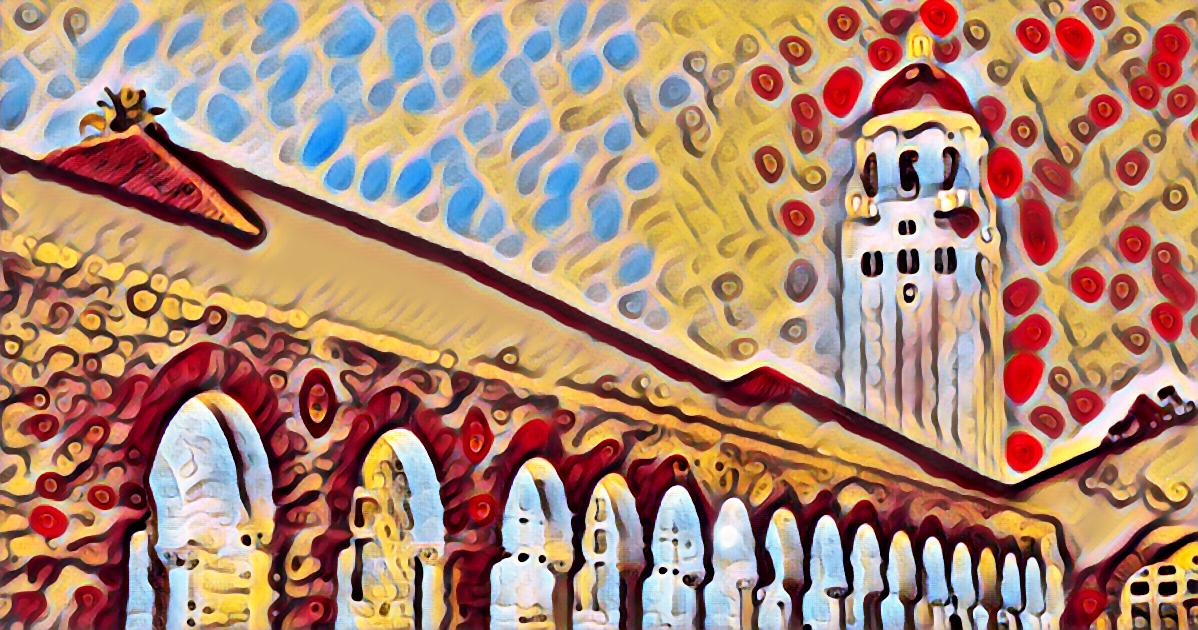
\includegraphics[height=0.20\textheight]{./img/jhonson_result_tower_candy.jpg}}
      
    \end{center}
  \end{figure}  
\end{frame}	
  
  
\section{Aprendizaje Automatico}
\iffalse
\begin{frame}
  \frametitle{Aprendizaje Automatico}
  \begin{itemize}
    \item Se encuentra en la intersección de las Cs. de la computación y el aprendizaje estadístico
    \item Aprendizaje supervisado vs no supervisado: etiquetas 
  \end{itemize}

  \begin{figure}[h]
    \begin{center}
      \subfloat[Clasificacion lineal]{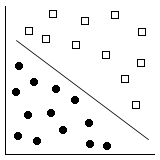
\includegraphics[height=0.20\textheight]{./img/linear_svm.png} \\
      \subfloat[Clustering]{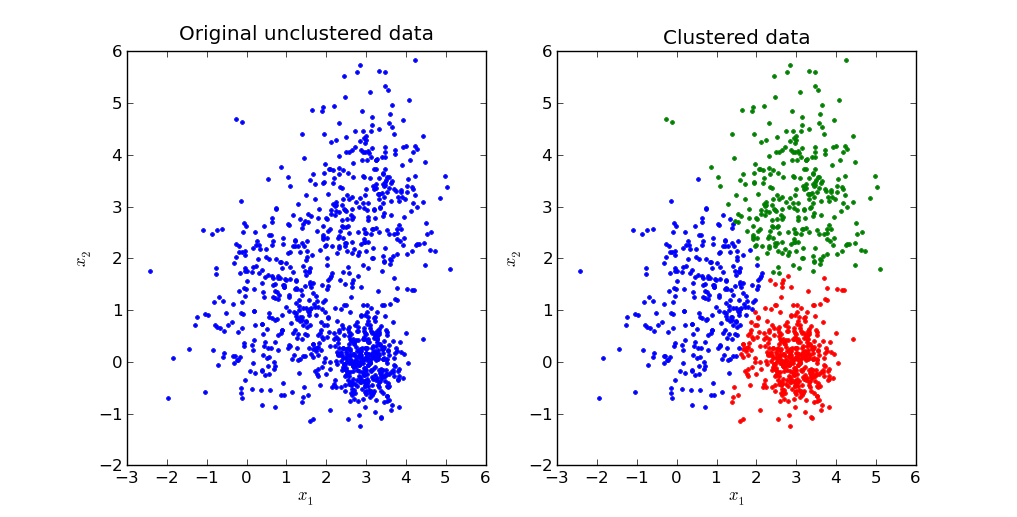
\includegraphics[height=0.20\textheight]{./img/stackoverflow_clustering.png}
    \end{center}
  \end{figure}  
\end{frame}
\fi
\begin{frame}
  \frametitle{Clasificacion de imagenes}
  \begin{itemize}
    \item Representación de la información: Features
    \item Enfoque clásico vs enfoque aprendizaje profundo
      \subitem Enfoque clásico: features predefinidas (Bag of Words) para entrenar el modelo
      \subitem Enfoque aprendizaje profundo: Tanto las features como el modelo se entrenan en conjunto 
  \end{itemize}
\end{frame}

\begin{frame}
  \frametitle{En que consiste el aprendizaje?}
  \begin{itemize}
    \item Funcion de predicción: mapeo $f_{\theta}: \mathcal{X} {\rightarrow} \{1,\dots,K\}$
    \item Objetivo del aprendizaje: minimizar $\theta$
    \item Optimización: minimizar función de pérdida (diferencia entre la predicción y el valor esperado)
  \end{itemize}
\end{frame}

\begin{frame}
  \frametitle{Descenso por el gradiente}
    Optimizar mediante refinamiento iterativo, siguiendo la dirección del gradiente de la función de pérdida.
    \begin{equation}
      w_{n+1} = w_n - \eta \nabla L(w_n)  = w_n - \eta \sum_{i=1}^{N} \nabla L_i(w_n)
    \end{equation}
\end{frame}

\section{Redes Neuronales Artificiales}
\begin{frame}
  \frametitle{Redes Neuronales Artificiales}
    \begin{itemize}
      \item Versión compleja de un clasificador lineal, utilizando funciones no lineales.
      \item Conjunto de unidades de cómputo (neuronas) conectadas en un grafo acı́clico organizadas por capas. 
      \item Las unidades de una capa se conectan con neuronas de sus capas adyacentes pero nunca se conectan 2 unidades de una misma capa.
    
    \end{itemize}

    
    \begin{figure}[ht]
      \begin{center}
	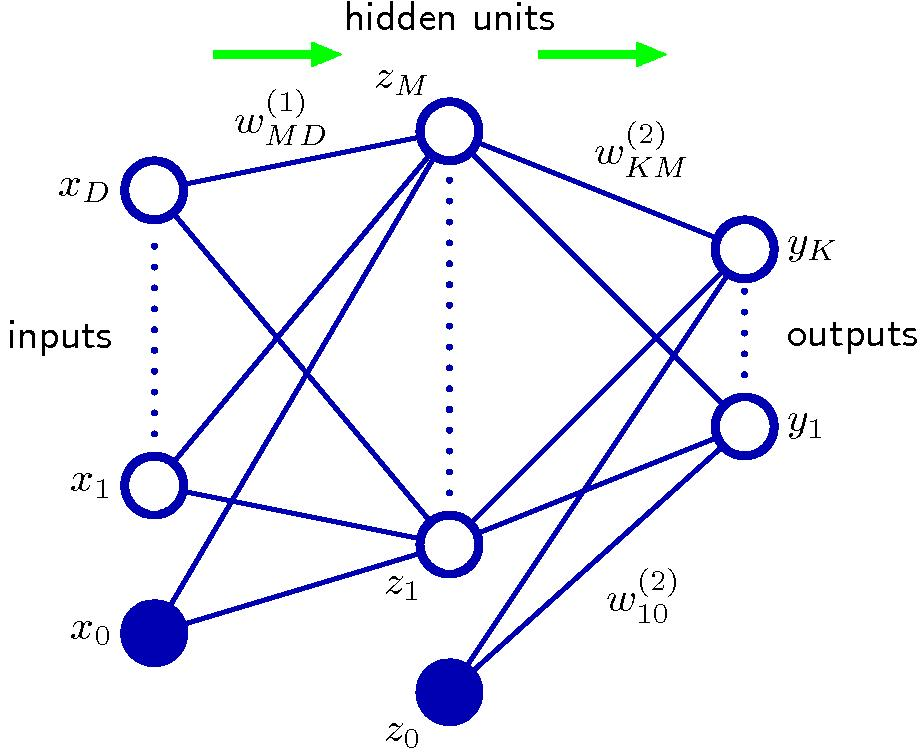
\includegraphics[width=0.8\linewidth]{./img/bishop_neural_network.jpg}
      \end{center}
      \caption{Red Neuronal Artificial}
    \end{figure}
\end{frame}

\begin{frame}
    \frametitle{Entrenando una red neuronal}
    Ciclos de 2 pasos
    \begin{enumerate}
      \item Paso hacia adelante: evaluación de la red en base al dato de entrada
      \item Retropropagación: corrección de los pesos internos de la red, según el gradiente de la función de pérdida.
    \end{enumerate}

    \begin{figure}[ht]
      \begin{center}
      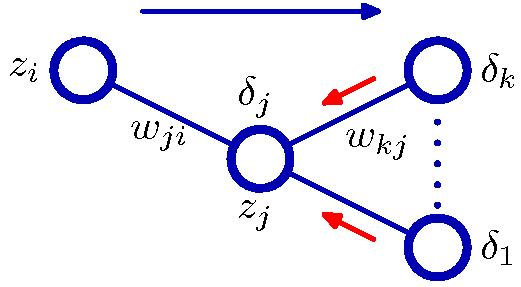
\includegraphics[width=0.5\linewidth]{./img/bishop_backpropagation.jpg}
      \end{center}
    \end{figure}
\end{frame}


\section{Redes Neuronales Convolucionales}
\begin{frame}
  \frametitle{Redes Neuronales Convolucionales - CNN}
    Redes Neuronales que asumen que sus entradas son imágenes
    \begin{itemize}
      \item Codificar propiedades en la arquitectura de la red:
	\subitem Localidad espacial
	\subitem Convolucion
	\subitem Submuestreo
    \end{itemize}
    
\end{frame}
  
\begin{frame}
  \frametitle{Funcion de convolucion}
    Se aplica un filtro (matriz de 3x3 o 5x5) desplazandolo por toda la imagen.
    Se obtiene una nueva imagen resultante de aplicar el filtro
    \begin{figure}[h]
      \begin{center}
      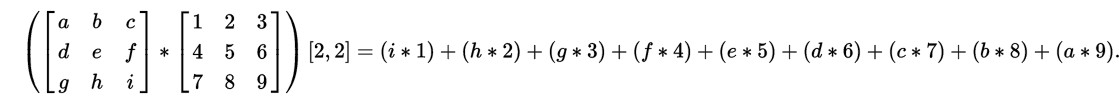
\includegraphics[width=\textwidth]{./img/convolution_wiki.jpg}
      \end{center}
    \end{figure}
\end{frame}
  
\begin{frame}
  \frametitle{Estructura de la CNN}
    \begin{itemize}
     \item Capa de Entrada
     \item Capa de Convolución
     \item Capa de Activación (No lineal)
     \item Capa de Submuestreo
     \item Capa de Salida
    \end{itemize}
  Los resultados intermedios entre cada una de las capas de los conoce como mapas de caracteristicas o feature maps.
  \begin{figure}[H]
    \begin{center}
      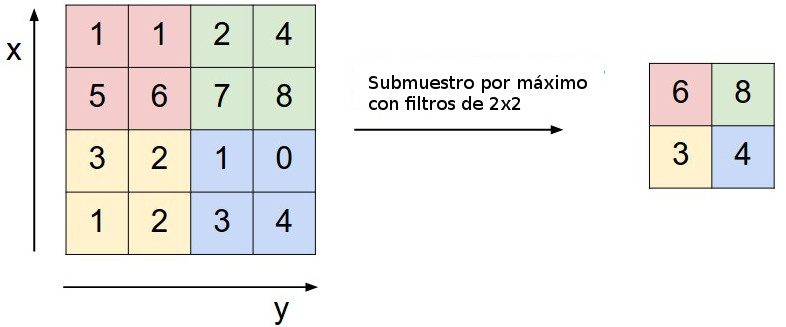
\includegraphics[width=0.8\linewidth]{./img/stanford_maxpool_spanish.jpeg}
    \end{center}
  \end{figure}
      
  \begin{figure}[h]
    \begin{center}
    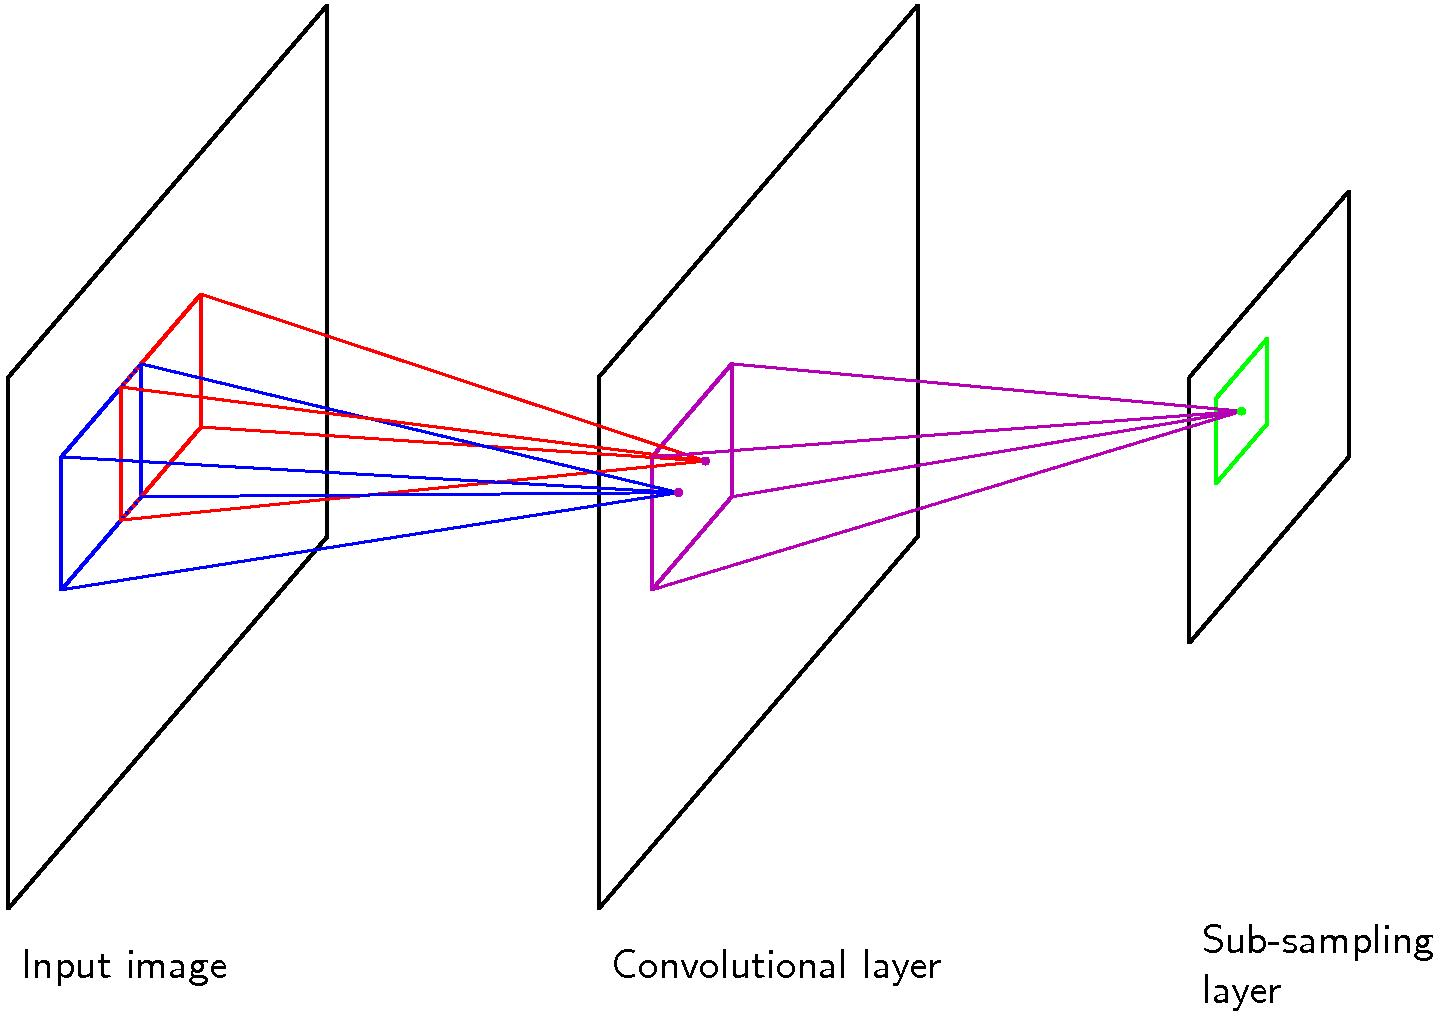
\includegraphics[width=0.8\linewidth]{./img/bishop_cnn.jpg}
    \end{center}
    \caption{Estructura de la CNN}
  \end{figure}
\end{frame}

\section{Ajuste Fino}
\begin{frame}
  \frametitle{Ajuste Fino - Finetuning}
    \begin{itemize}
     \item Adaptar una red preentrenada a un problema similar
     \item Toma una red preentrenada y un pequeno conjunto de datos
     \item Reemplaza la ultima capa adaptada al problema
     \item Reentrena la red comenzando con los pesos predefinidos, ajustandolos a los nuevos datos
    \end{itemize}
\end{frame}


\section{Algoritmo de transferencia de estilo}
\begin{frame}
 \frametitle{Algoritmo de transferencia de estilo}
 \begin{itemize}
    \item Algoritmo publicado por Gatys et. al.
    \item Toma como entrada 2 imágenes: una de contenido y otra de estilo
    \item Partiendo de una imagen de ruido, genera iterativamente una imagen artificial, compuesta por el contenido de una imagen y el estilo de la otra.
    \item Utiliza los mapas de caracteristicas de CNN para calcular el estilo y el contenido.
 \end{itemize}
  \begin{figure}[h]
    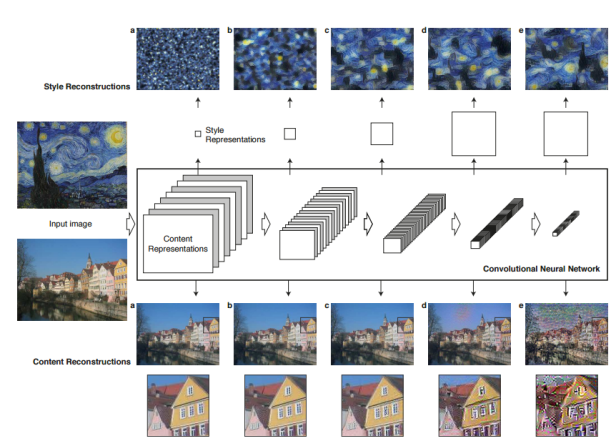
\includegraphics[width=\textwidth]{./img/gatys_1.png}
    \caption{Reconstrucciones del Estilo y Contenido utilizando una CNN}
  \end{figure} 
\end{frame}

\begin{frame}
 \frametitle{Contenido}
  \begin{itemize}
   \item Representación del contenido: mapa de caracteristicas de una de las ultimas capas de la red.
   \item Mapa de caracteristicas de la imagen de contenido: matriz $F^l \in R^{N_l \times M_l}$, donde $F_{i,j}^l$ es la respuesta del $i$-esimo filtro en la posición $j$.
   \item Función de pérdida del contenido: Error cuadrático medio entre los mapas de caracteristicas de la imagen generada $F$ y la imagen de contenido $P$.
  \end{itemize}
  \begin{equation}
    L_{contenido}(\overrightarrow{p},\overrightarrow{x}, l) = \frac{1}{2} \sum_{i,j} (F_{i,j}^l - P_{i,j}^l)^2
  \end{equation}
\end{frame}

\begin{frame}
 \frametitle{Estilo}
  \begin{itemize}
    \item Representación del estilo: correlación entre los valores del mapa de caracteristicas.
    \item Correlación de caracteristicas: $G^l \in R^{N_l \times N_l}$, en la cual $G_{i,j}^l$ se calcula como el producto punto entre los vectores
      de los mapas de características $i$ y $j$ en la capa $l$:
	\begin{equation}
	  G_{i,j}^l = \sum_{k} F_{i,k}^l F_{j,k}^l
	\end{equation}
    \item Función de pérdida del estilo: Suma pesada de los errores entre el estilo calculado de la imagen generada y la imagen de estilo, de varias capas.
  \end{itemize}
  La contribución de esa capa a la función de pérdida total del estilo es:
      \begin{equation}
       E_l = \frac{1}{4 N_l^2 M_l^2} \sum_{i,j} (G_{i,j}^l - A_{i,j}^l)^2
      \end{equation}
      De esta forma, la función de pérdida del estilo total queda definida como una combinación lineal de las funciones de pérdida de estilo de cada capa:
      \begin{equation}
       L_{estilo}(\overrightarrow{a},\overrightarrow{x}) = \sum_{l=0}^{L} w_l E_l
      \end{equation}
\end{frame}

\begin{frame}
  \frametitle{Transferencia de estilo}
  Función de pérdida total: 
      \begin{equation}
	L_{total}(\overrightarrow{p},\overrightarrow{a},\overrightarrow{x}) = \alpha L_{contenido}(\overrightarrow{p},\overrightarrow{x}) + \beta L_{estilo}(\overrightarrow{a},\overrightarrow{x})
      \end{equation}
  \begin{figure}[h]
    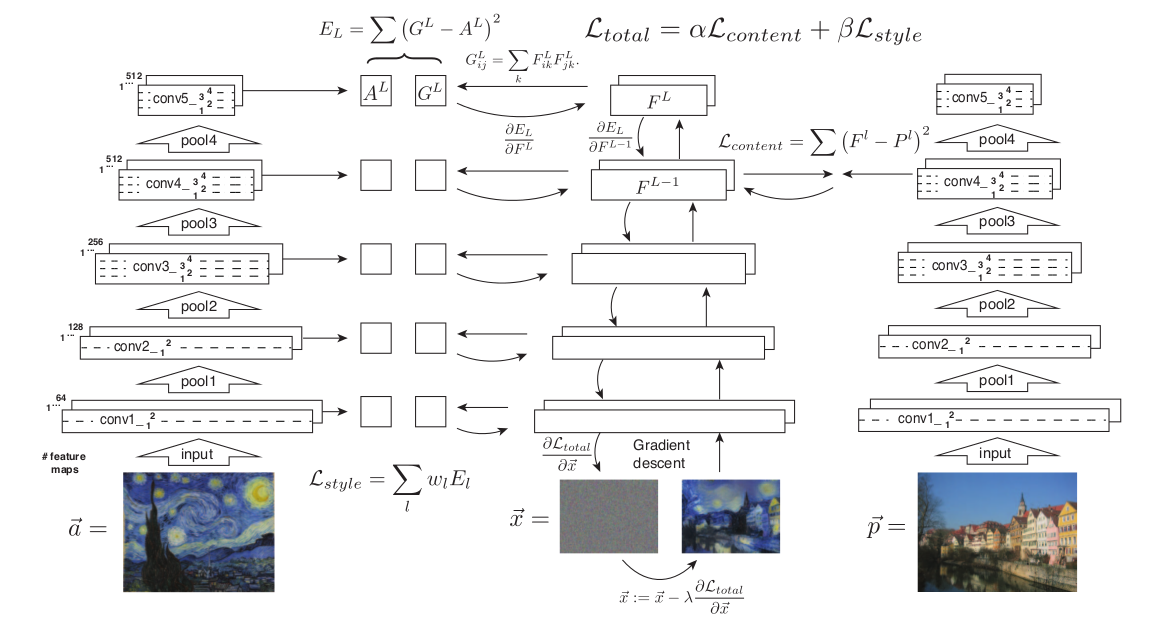
\includegraphics[width=\textwidth]{./img/gatys_method.png}
    \caption{Algoritmo de transferencia de estilo}
  \end{figure}
\end{frame}

\begin{frame}
  \frametitle{Hiperparámetros}
  \begin{itemize}
   \item Número de iteraciones: Determina cuantas veces se ejecuta el método de descenso por el gradiente para minimizar la función de pérdida. 
   \item Red Convolucional: Dependiendo de la red convolucional que se utilice, cambia el tamaño de los mapas de características, las capas, etc.
   \item Capas de la red para la representación de estilo y sus respectivos pesos ($w_l, l \in \{1 \dots L\}$).
   \item Capa de la red para la representación del contenido.
   \item Factores de peso para las funciones de pérdida de estilo y contenido en la función de pérdida total $(\alpha, \beta)$.
   \item otros..
  \end{itemize}

\end{frame}


\section{Elección automática de hiperparámetros}
\begin{frame}
  \frametitle{Problema: elección automática de hiperparámetros}
  \begin{itemize}
   \item El número de iteraciones se detectó como el principal factor de influencia en el resultado del algoritmo.
   \item En el arte, las evaluaciones suelen ser cualitativas.
    \subitem Es necesario definir un criterio cuantitativo de evaluación para poder determinar si un resultado es aceptado o no.
  \item Objetivo: generar una imagen aceptada en la menor cantidad de iteraciones posible.
  \end{itemize}

\end{frame}

\begin{frame}
 \frametitle{Solución propuesta}
  \begin{itemize}
   \item Módulo de generación de imágen: transferencia de estilo
   \item Módulo de evaluación: reconocimiento de estilo
   \item Definir critero de aceptación cuantitativo: estilo cercano a la imagen objetivo 
  \end{itemize}
  \begin{figure}[h]
    \begin{center}
      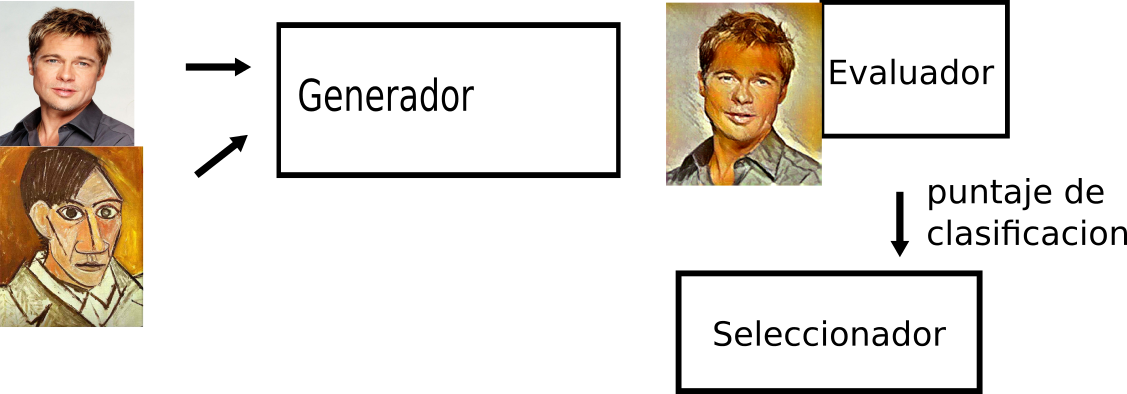
\includegraphics[width=\linewidth]{./img/diagrama.png}
    \end{center}
    \caption{Diagrama de interacción entre los distintos módulos propuestos}
  \end{figure}
\end{frame}

\section{Experimentos}
\begin{frame}
  \frametitle{Reconocimiento de estilo}
  \begin{itemize}
    \item Finetuning sobre red preentrenada para clasificar objetos
    \item Datos provenientes de WikiArt.
    \item POC sobre los 10 principales estilos
  \end{itemize}
\end{frame}

\begin{frame}
  \frametitle{Estilos}
  \begin{figure}
      \begin{center}
      \def\tabularxcolumn#1{m{#1}}
      \begin{tabularx}{\textwidth}{@{}cXX@{}}
      %
      \begin{tabular}{cc}
	\subfloat[Modernismo]{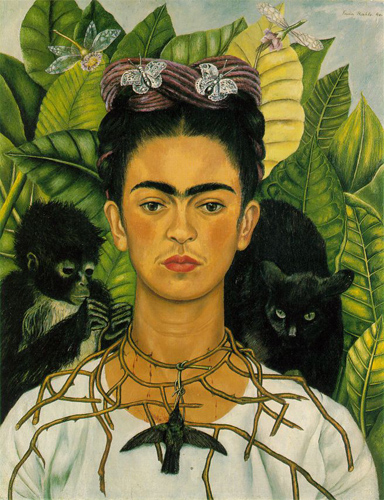
\includegraphics[height=0.15\textheight]{./img/frida_kahlo.jpg}}
	& \subfloat[Impresionismo]{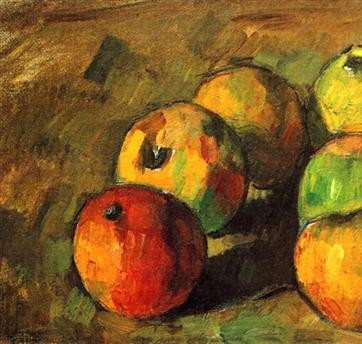
\includegraphics[height=0.15\textheight]{./img/cezanne.jpg}}\\
	\subfloat[Surrealismo]{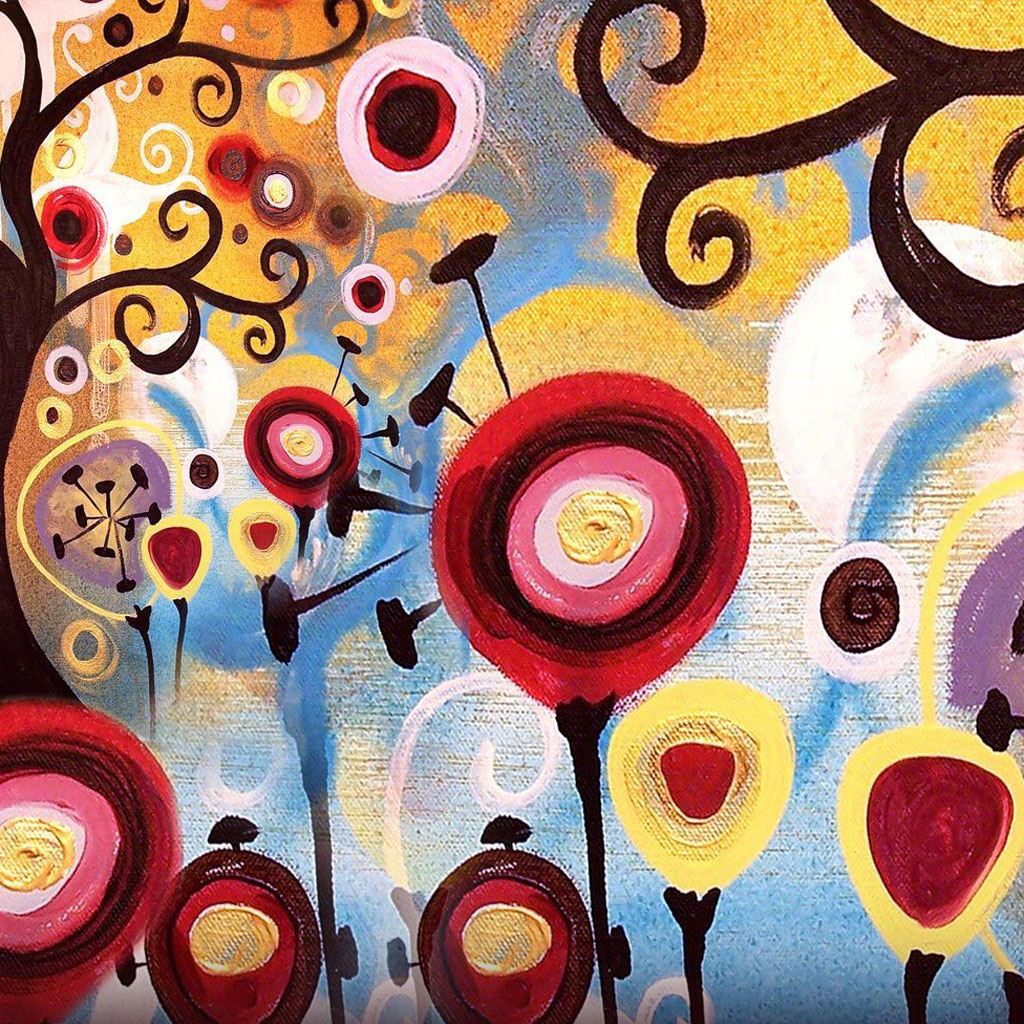
\includegraphics[ height=0.15\textheight]{./img/jhonson_style_candy.jpg}}
	& \subfloat[Post Impresionismo]{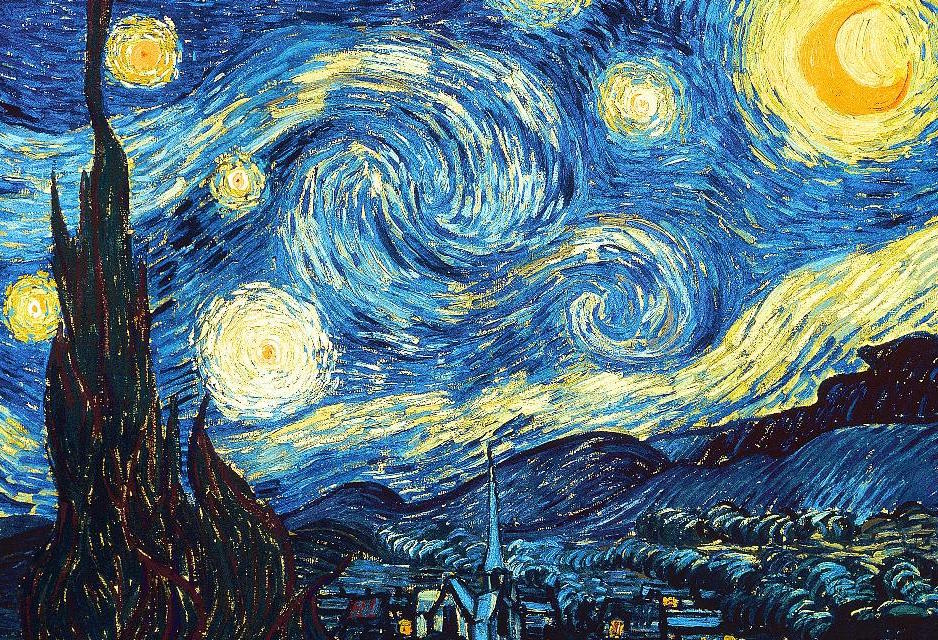
\includegraphics[height=0.15\textheight]{./img/starry_night.jpg}}\\
	\subfloat[Simbolismo]{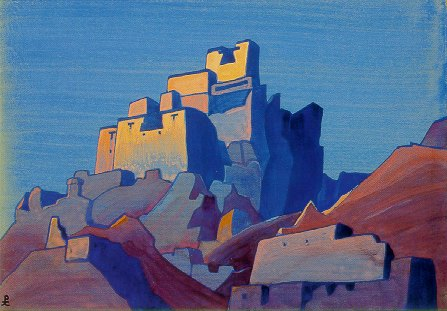
\includegraphics[ height=0.15\textheight]{./img/nicholas-roerich_chiktan-citadel-in-himalayas.jpg}}
	& \subfloat[Neo Clasisimo]{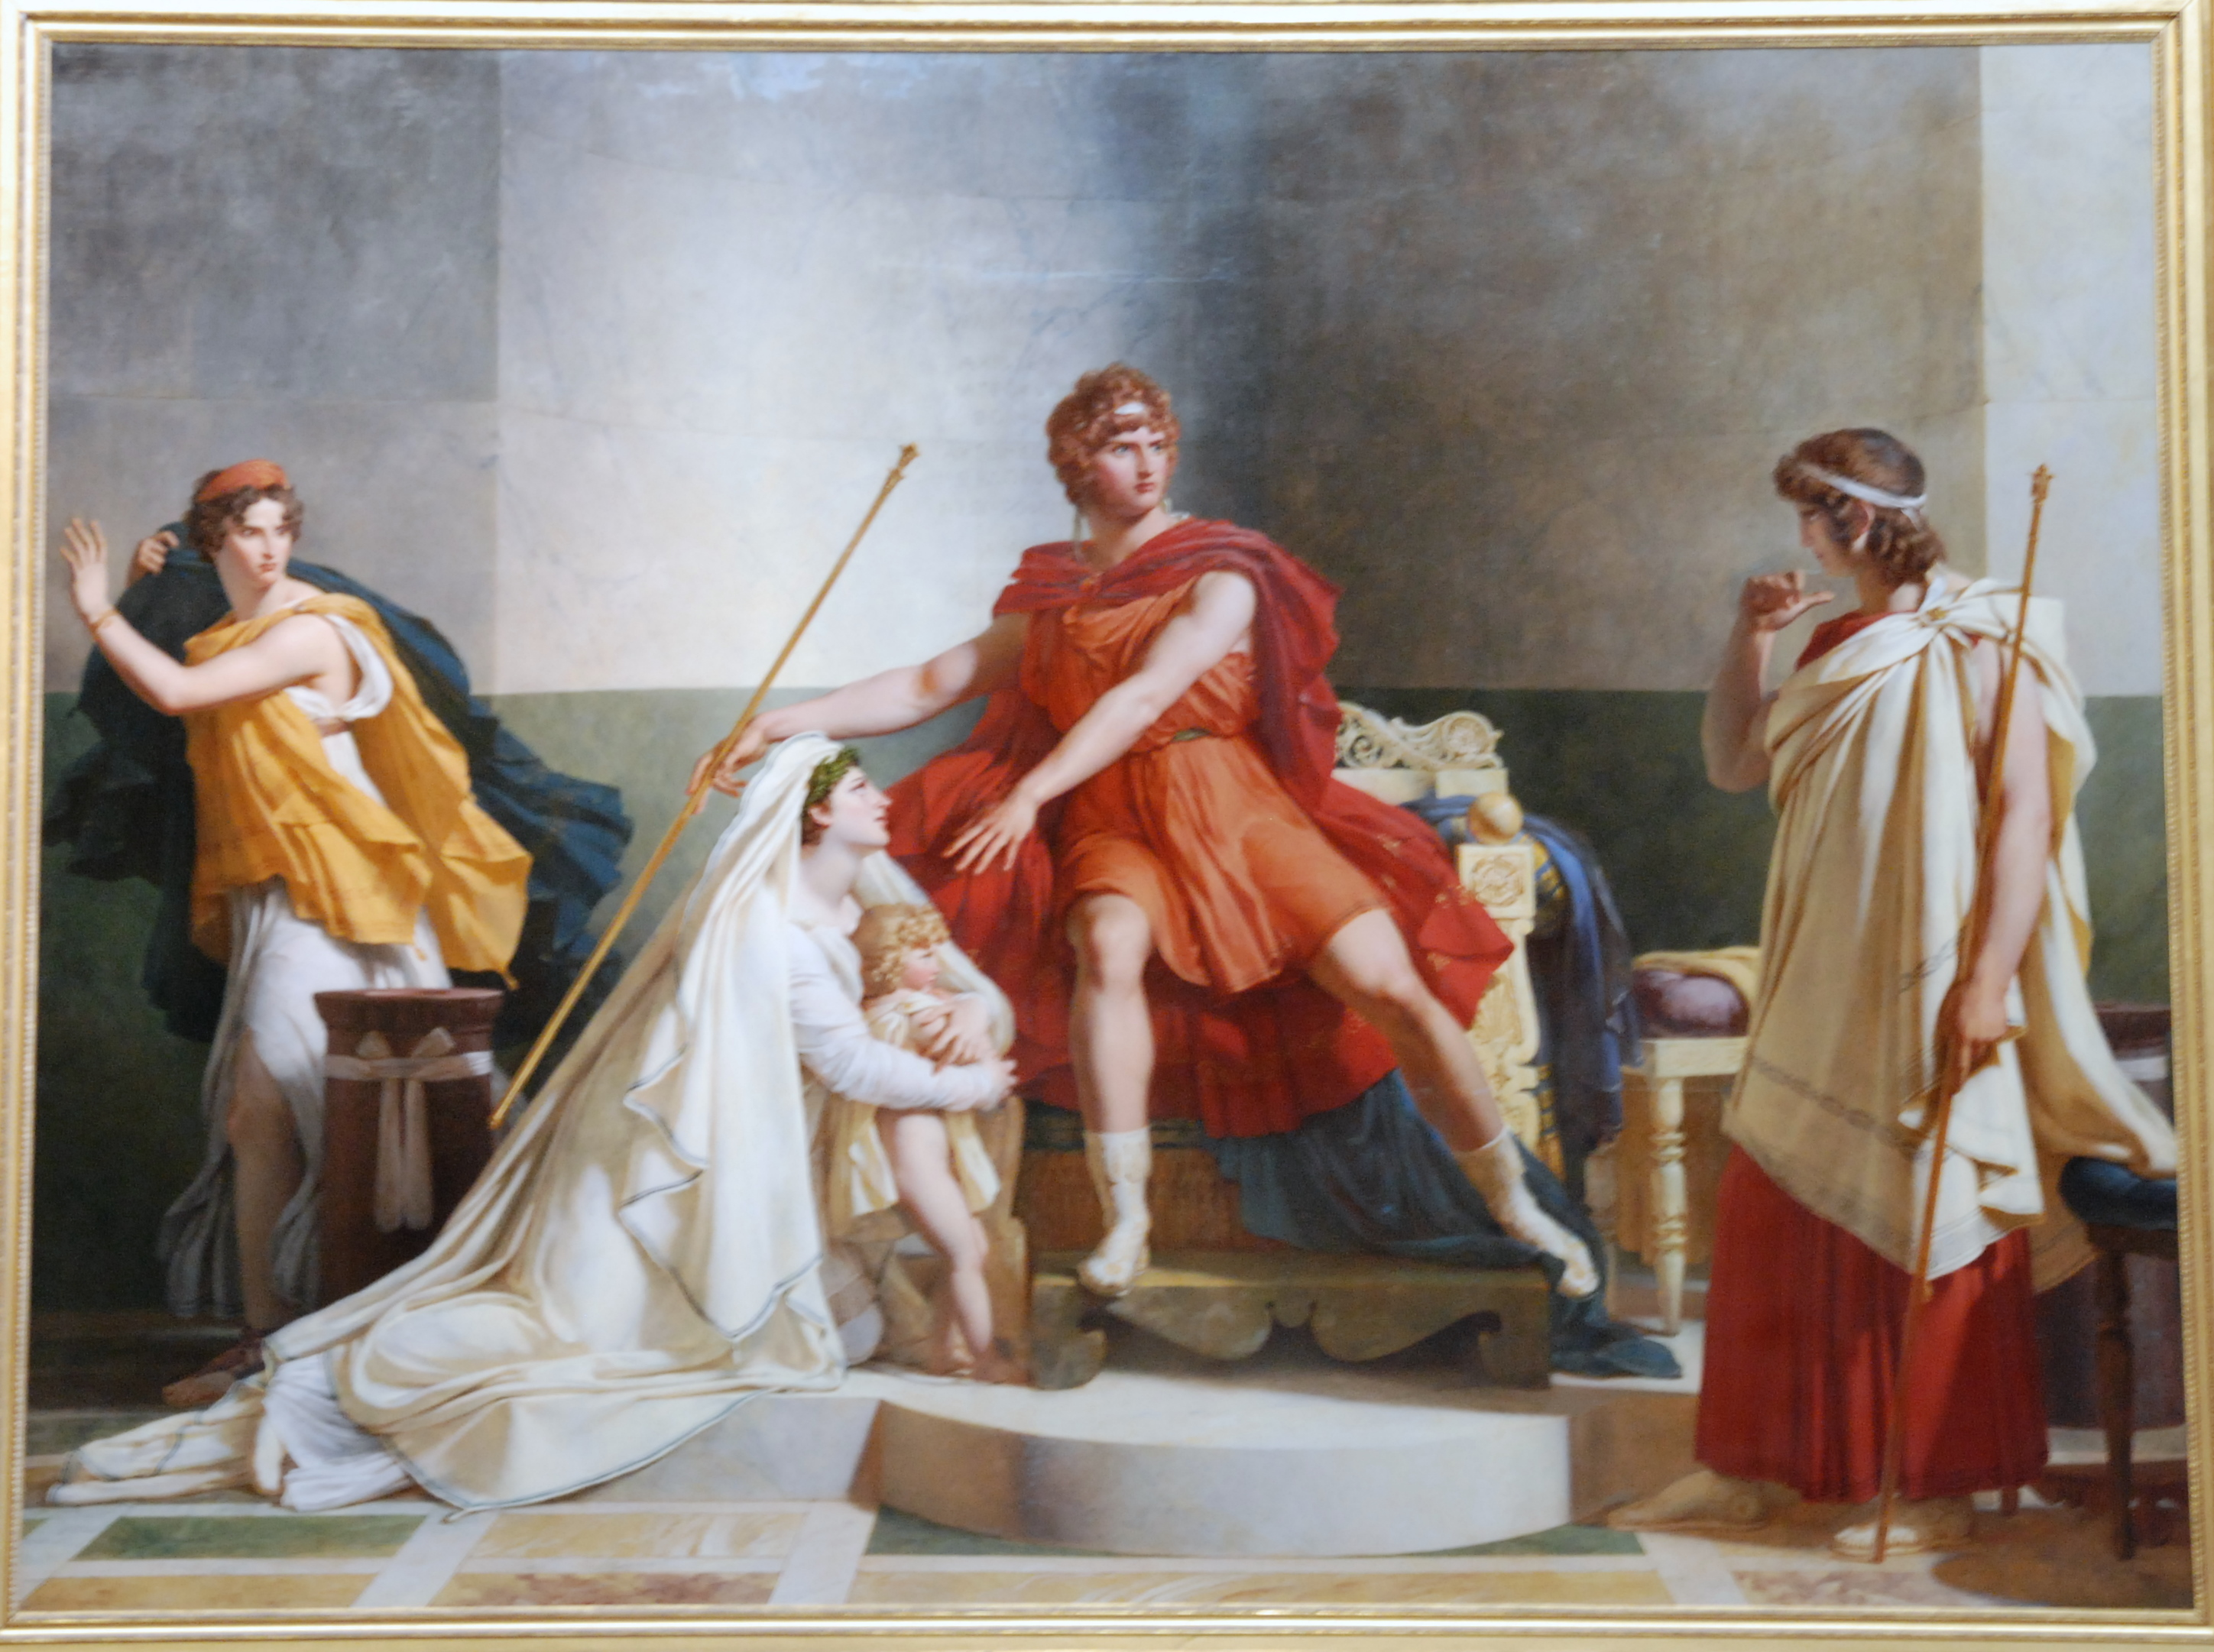
\includegraphics[height=0.15\textheight]{./img/pierre-narcisse-guerin_not-detected.jpg}}\\
	\subfloat[Romanticismo]{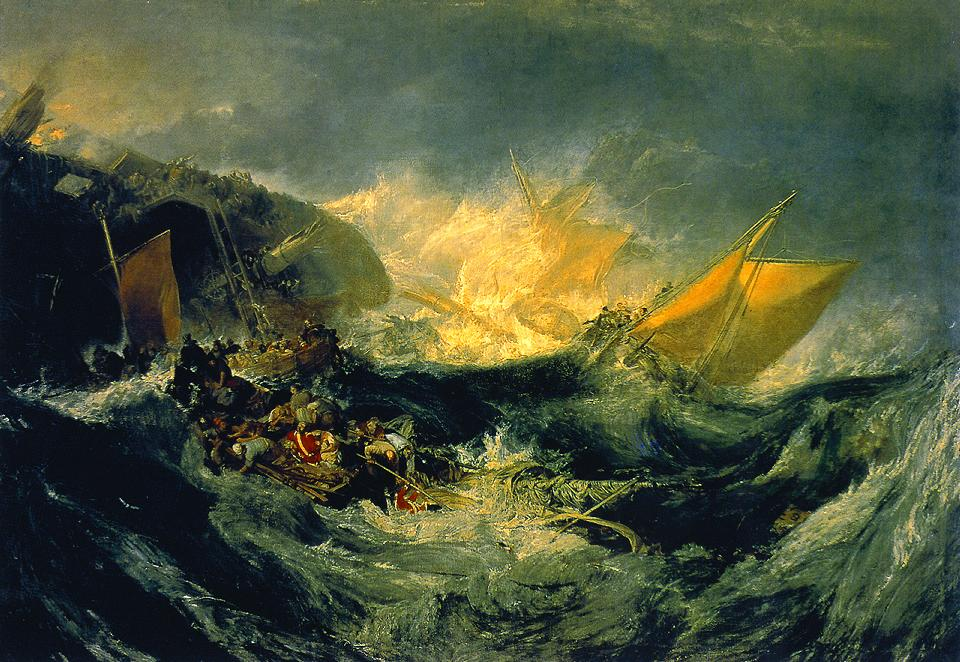
\includegraphics[height=0.15\textheight]{./img/shipwreck.jpg}}
	& \subfloat[Barroco]{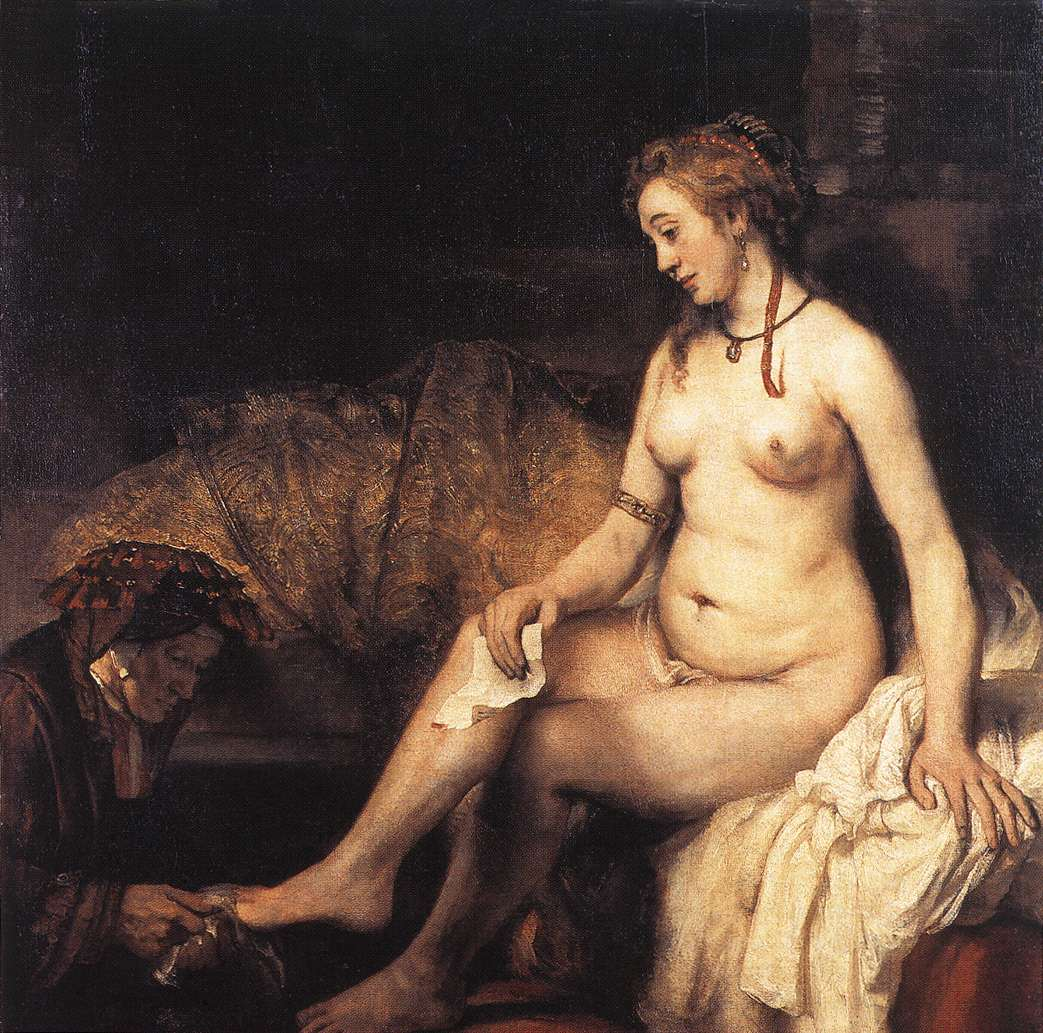
\includegraphics[height=0.15\textheight]{./img/rembrandt_bathsheba-bathing.jpg}}\\
	\subfloat[Realismo]{\includegraphics[height=0.15\textheight]{./img/vincent-van-gogh_cart-with-red-and-white-ox.jpg}}
	& \subfloat[Expresionismo]{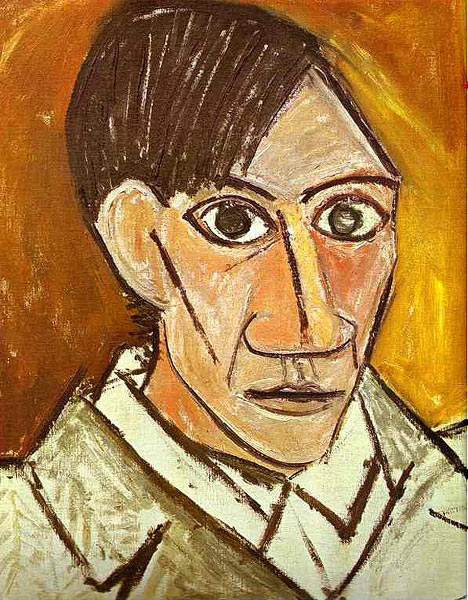
\includegraphics[height=0.15\textheight]{./img/picasso_selfport.jpg}}\\
      \end{tabular}

      \end{tabularx}

      \caption{Ejemplos de obras de arte correspondientes a los estilos seleccionados}\label{mosaico_estilos}
      \end{center}

    \end{figure}
\end{frame}

\begin{frame}
  \frametitle{Elección del número de iteraciones}
  Se detectaron 2 situaciones distintas en los resultados obtenidos:
  \begin{itemize}
    \item El estilo de la imagen resultante coincide con el estilo de la imagen obtenida
    \item El estilo de la imagen resuttante NO coincide con el estilo de la imagen obtenida
  \end{itemize}

\end{frame}

\begin{frame}
  \frametitle{Caso 1}
\end{frame}

\begin{frame}
  \frametitle{Caso 2}
\end{frame}

\begin{frame}
  \frametitle{Analisis criterio de aceptación planteado}
  En base a los resultados obtenidos, se determinó que el criterio inicialmente planteado no es válido.
  El criterio utilizado fue determinar numero de iteraciones el punto medio del periodo donde alcanza un mayor puntaje de reconocimiento de estilo
\end{frame}

\section{Conclusiones}
\begin{frame}{Conclusiones}
%%%%%%%
\end{frame}



\begin{frame}
 {\Huge ¿Preguntas?}
\end{frame}

\begin{frame}
 {\Huge ¡Gracias por escuchar!}
\end{frame}


\end{document}
